\documentclass{article}

% Language setting
% Replace `english' with e.g. `spanish' to change the document language
\usepackage[english]{babel}

% Set page size and margins
% Replace `letterpaper' with `a4paper' for UK/EU standard size
\usepackage[letterpaper,top=2cm,bottom=2cm,left=3cm,right=3cm,marginparwidth=1.75cm]{geometry}

% Useful packages
\usepackage{amsmath}
\usepackage{graphicx}
\usepackage[colorlinks=true, allcolors=blue]{hyperref}
\usepackage{algorithm}
\usepackage{algpseudocode}
\usepackage{float}

\title{Implementation of Reinforcement Learning and Deep Reinforcement
Learning algorithms in Multi-Agent Systems for Autonomous Vehicle
Coordination}
\author{
Edonisa Dautaj\\[0.2cm]
Supervised by Dr. Maxime Guériau and Fatima-Ezzahra Maad\\
\small INSA Rouen Normandie, LITIS UR 4108, France
}

\begin{document}
\maketitle

\begin{center}
\textbf{Abstract}
\end{center}

\noindent
This paper studies the use of reinforcement learning and deep reinforcement learning techniques for autonomous vehicle coordination in simulated traffic environments using SUMO. The work is based on an existing simulation framework that already included Q-Learning and DQN implementations. The main contribution of this work was to extend the existing codebase by adding DDQN and PPO. For DDQN, the existing DQN structure was adapted, while PPO was implemented as a separate actor-critic model based on policy-gradient learning.

\section{Introduction}

Autonomous driving is an important research area within intelligent transportation systems, where vehicles are expected to make safe and efficient decisions in changing traffic conditions. One of the main challenges is decision-making in situations where vehicles must interact with other road users, such as unsignalized intersections and highway ramp merging. In these scenarios, the vehicle has to choose suitable actions while taking into account both safety and traffic flow.

Reinforcement learning provides a useful framework for this type of sequential decision-making problem. In reinforcement learning, an agent learns through interaction with an environment by selecting actions and receiving rewards or penalties based on the consequences of those actions \cite{sutton2018reinforcement}. This is relevant for autonomous driving because the behavior of the vehicle does not need to be fully hand-coded; instead, the agent can learn a driving policy through repeated simulation.

Deep reinforcement learning extends this idea by combining reinforcement learning with neural networks. Neural networks are useful when the state representation becomes more complex, because they can approximate functions instead of relying only on explicit tables \cite{goodfellow2016deep}. This makes deep reinforcement learning suitable for traffic simulation problems where the environment may include different road structures, vehicle interactions, and decision conditions.

This project uses SUMO as the traffic simulation environment. SUMO is an open-source microscopic traffic simulator commonly used for modeling road networks, vehicle movement, and traffic-related experiments \cite{behrisch2011sumo}. This project uses SUMO to study reinforcement learning methods for autonomous vehicle coordination and to test additional learning approaches within the existing experimental framework.

\section{Problem Statement}

The main problem addressed in this project is the limited ability of reinforcement learning agents to remain reliable when the traffic scenario changes. A policy trained in one environment may not perform equally well when the road structure, vehicle interactions, or decision conditions are different.

This is important because training a new agent from scratch for every new scenario can be inefficient. Instead, it is useful to study whether learned behavior can be reused, adapted, or improved when the environment changes. In this project, this problem is studied within a SUMO-based simulation framework by examining the existing learning pipeline and adding additional deep reinforcement learning methods for comparison.



\section{Related Work and Existing Approaches}

Previous research has used learning-based methods to study driving behavior in situations where fixed rules are difficult to define. In reinforcement learning, the problem is commonly described as choosing actions over time in order to maximize long-term reward \cite{sutton2018reinforcement}. This provides the theoretical basis for the value-based and policy-based methods discussed in this section.

The following subsections present Q-Learning, DQN, DDQN, and PPO, followed by transfer learning and policy fusion. The latter is especially relevant because the reference work by Maad et al. studies knowledge transfer between autonomous driving agents in SUMO scenarios involving T-intersections and ramp merges \cite{maad2025dynamic}.

\subsection{Reinforcement Learning Approaches}

Reinforcement learning studies how an agent can choose actions over time in order to maximize cumulative reward \cite{sutton2018reinforcement}. This formulation is commonly described using states, actions, rewards, and a policy that guides the agent's behavior.

In traffic simulation, this framework can be used to model a vehicle as the learning agent. The vehicle observes the current traffic situation, selects an action such as accelerating, maintaining speed, or decelerating, and receives feedback based on safety and efficiency. A similar formulation is used by Maad et al., where autonomous driving scenarios in SUMO are modeled using states, actions, and reward functions \cite{maad2025dynamic}.

\begin{figure}[h]
    \centering
    
\includegraphics[width=0.55\textwidth]{RS.drawio.png}
    \caption{Basic reinforcement learning interaction loop between the agent and the environment.}
    \label{fig:rl_loop}
\end{figure}


\subsubsection{Q-Learning}

Q-Learning is a value-based reinforcement learning algorithm \cite{sutton2018reinforcement}. The main idea is to learn the value of taking a certain action in a certain state. These values are called Q-values and are usually stored in a Q-table when the number of states and actions is limited. During training, the Q-values are updated using the reward received from the environment and the estimated value of the next state \cite{watkins1992qlearning}.

The update rule can be written as:

\[
Q(s_t,a_t) \leftarrow Q(s_t,a_t) + \alpha \left[r_t + \gamma \max_a Q(s_{t+1},a) - Q(s_t,a_t)\right]
\]

where $\alpha$ is the learning rate, $\gamma$ is the discount factor, $r_t$ is the reward, and $s_{t+1}$ is the next state.

Q-Learning is useful as a first reinforcement learning approach because it is relatively simple and easy to interpret. In this project, it is important because it is already included in the existing codebase and provides a baseline to understand how an agent can learn driving decisions in SUMO. However, tabular Q-Learning becomes less practical when the state space becomes large or more complex because the agent needs to store and update values for many possible state-action pairs.



\subsubsection{Deep Q-Network}

DQN extends Q-Learning by using a neural network to approximate Q-values instead of storing them in a table. This makes DQN more suitable for problems where the state representation is too large or too complex for a tabular method. The original DQN approach also introduced important techniques such as experience replay and target networks to improve training stability \cite{mnih2015human}.

In this project, DQN is relevant because it represents the deep reinforcement learning baseline in the existing SUMO codebase. It keeps the same general idea as Q-Learning, where the agent selects actions based on estimated Q-values, but it uses a neural network to estimate these values. Understanding DQN is also important because DDQN is built as an extension of the same general structure.


\subsubsection{Double Deep Q-Network}

DDQN is an extension of DQN that was introduced to reduce the overestimation of Q-values. In standard DQN, the same value estimation process can lead the agent to overestimate the value of some actions. DDQN addresses this by separating action selection from action evaluation when computing the target value \cite{vanhasselt2016deep}.

This makes DDQN a natural method to study after DQN. Since the existing project already contains a DQN implementation, DDQN can be added by modifying the way the target Q-value is computed, while keeping much of the general training pipeline similar. For this reason, DDQN is considered as one of the first extensions to implement in this project.

In this work, the DDQN implementation was developed by extending the existing DQN structure already present in the codebase. The main objective was to keep the general project pipeline consistent while modifying the learning logic of the agent. In particular, the state space, action space and reward structure were kept the same as in the DQN implementation, while the main change was introduced in the target Q-value computation in order to follow the DDQN approach.


\subsubsection{Proximal Policy Optimization}

PPO is a policy-gradient reinforcement learning method introduced to improve the stability of policy updates during training \cite{schulman2017proximal}. Unlike Q-Learning, DQN, and DDQN, which are value-based methods, PPO directly optimizes the policy used by the agent to select actions.

PPO is commonly implemented using an actor-critic structure. The actor is responsible for selecting actions, while the critic estimates the value of the current state. This type of structure is commonly used in policy-gradient methods because it combines policy learning with value estimation \cite{sutton2018reinforcement}.

A key idea of PPO is to avoid making policy updates that are too large. Instead of allowing the new policy to move too far from the previous one, PPO uses a clipped objective function to keep the update within a limited range. This makes training more stable and reduces the risk of sudden performance drops \cite{schulman2017proximal}.

In this project, PPO is relevant because it represents a different family of reinforcement learning methods compared to Q-Learning, DQN, and DDQN. While the previous methods are value-based, PPO follows a policy-gradient approach, which makes it useful for comparing different learning strategies in the same traffic simulation setting.


\subsection{Transfer Learning and Policy Fusion Approaches}

This project is related to recent work on knowledge transfer between autonomous driving agents, especially the framework proposed in \textit{Knowledge Transfer via Dynamic Policy Fusion between Autonomous Driving Agents}. In that work, a source agent trained in one traffic scenario can help a target agent adapt to a new environment by sharing useful knowledge, instead of forcing the target agent to rely only on random exploration \cite{maad2025dynamic}.

More generally, transfer learning in reinforcement learning aims to reuse knowledge learned in one task in order to improve learning or adaptation in another task. In autonomous driving, this is important because training a completely new agent from scratch for every scenario can be inefficient. A policy learned in one environment may still contain useful decision-making knowledge for another related environment \cite{maad2025dynamic}.

In the paper by Maad et al., this idea is studied through two traffic scenarios: T-intersection navigation and ramp merging. The authors compare zero-shot transfer, basic transfer learning, and transfer learning with fine-tuning. Their main contribution is a dynamic policy fusion mechanism, where the target agent combines its own Q-values with those of the source agent. At the beginning, the source policy has more influence, and later the target agent gradually relies more on its own learned behaviour \cite{maad2025dynamic}.

This approach is relevant for the current project because it shows how previously learned policies can support adaptation across traffic scenarios. It also provides an important research direction for studying whether autonomous driving agents can generalize more efficiently when knowledge from another trained agent is available \cite{maad2025dynamic}.

\section{Methodology}
This section describes the main reinforcement learning setup used in the project. Since the work is based on an existing SUMO framework and later extended with additional algorithms, it is important to clearly describe the state space, action space, reward design, and evaluation metrics used during the experiments. When an implementation keeps the same environment settings as previous models, this is also stated explicitly, so that the differences between algorithms remain clear.

\subsection{Reinforcement Learning Setup}

The learning setup used in this project is based on a SUMO traffic simulation controlled through Python and TraCI. Each experiment focuses on one controlled vehicle, represented by its vehicle ID, route, color, and SUMO configuration file. The agent observes the traffic situation, selects an action, and receives a reward from the environment after each simulation step.

The same general simulation pipeline is used across the different algorithms in order to keep the comparison consistent. The SUMO command includes collision warnings, junction collision checking, a step length of 0.1 seconds, and automatic simulation start. These settings are used in the training and validation scripts for the different agents.

In the original framework, Q-Learning and DQN were already available. In this work, DDQN and PPO were added using the same general experimental structure. DDQN follows the DQN-style training pipeline with a policy network, target network, replay memory, and saved model weights, while PPO uses a separate actor-critic implementation and stores episode trajectories before updating the policy.

\subsection{State Space and Action Space}

The project uses two types of state representations, depending on the learning algorithm. For the tabular Q-Learning setup and the PPO implementation, the environment is represented using five discrete states. These states describe the current driving situation using color-based categories: black for collision or highly dangerous situations, red for risky navigation, orange for warning situations, green for safe navigation, and white for successful goal achievement. This follows the same general discretization idea used in the original SUMO framework, where the vehicle state is classified according to safety conditions such as distance to the leading vehicle, speed, and goal completion \cite{maad2025dynamic}.

\begin{figure}[H]
    \centering
    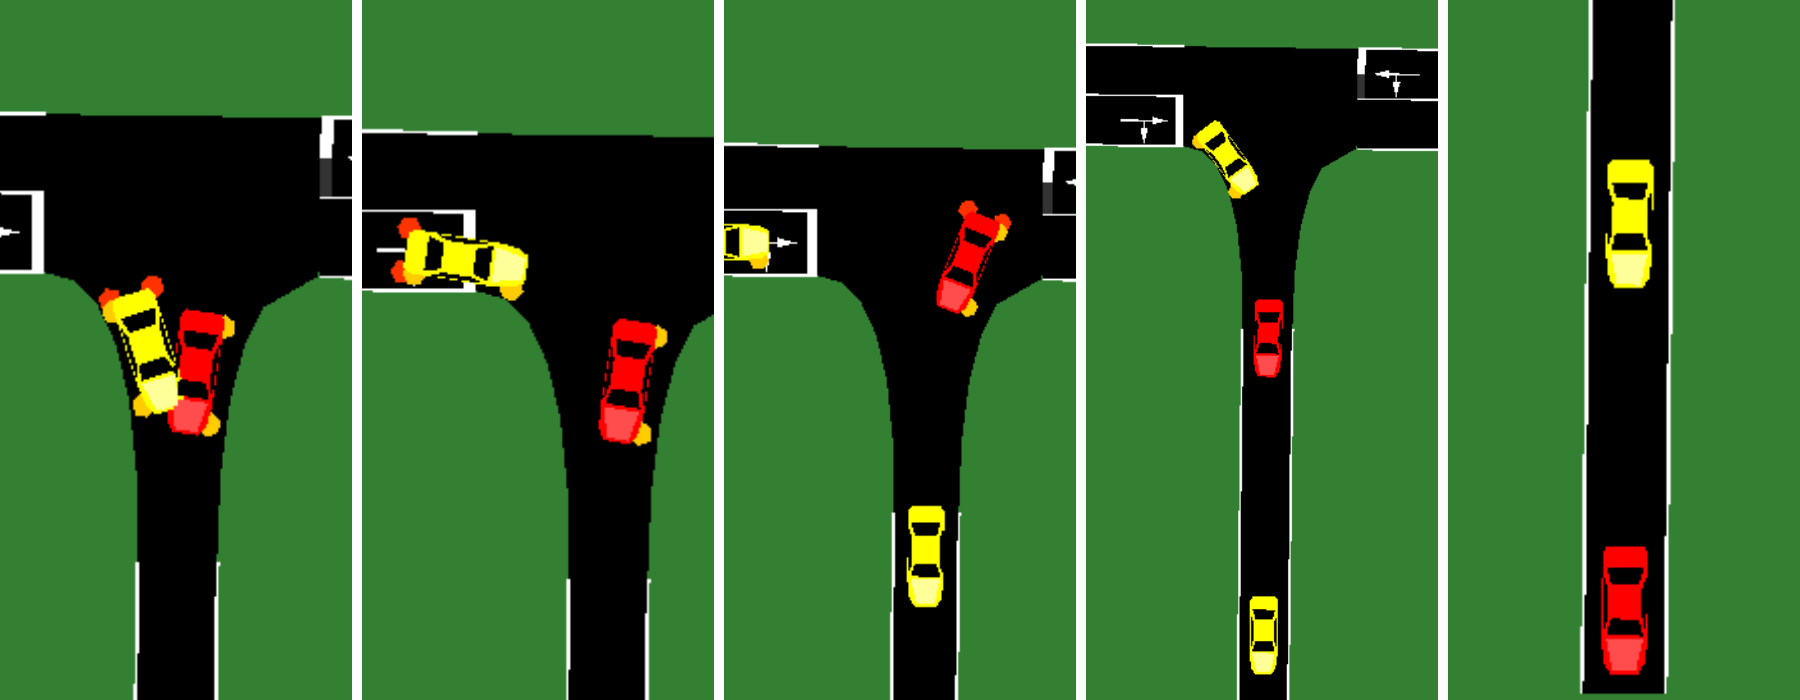
\includegraphics[width=\textwidth,keepaspectratio]{figures/states.png}
    \caption{Illustrative examples of the discrete state categories used in the SUMO environment: black for collision or highly dangerous situations, red for risky navigation, orange for warning situations, green for safe navigation, and white for successful route completion.}
    \label{fig:state_examples}
\end{figure}



\noindent
For DQN and DDQN, the state representation is different because these methods use neural networks instead of a table. In this case, the state is represented as a numerical vector containing the vehicle speed, the distance gap to the leading vehicle, and the accumulated waiting time. These values are normalized before being passed to the network, so that the model receives a compact continuous representation of the traffic situation.

The action space is kept discrete across all implemented models. At each decision step, the agent can choose between three possible actions: accelerate, maintain the current behavior, or decelerate. Keeping the same action space makes the comparison between Q-Learning, DQN, DDQN, and PPO more consistent, since the algorithms differ mainly in how they learn from the environment rather than in the set of actions available to the vehicle.

\subsection{Reward Function}

The reward function is designed to guide the vehicle toward safe and efficient driving behavior. The same general reward logic is used across the implemented agents, so that the comparison between algorithms is based mainly on the learning method rather than on different reward definitions.

The reward penalizes unsafe situations such as collisions, very small distance gaps, risky navigation, and excessive waiting time. In contrast, it gives positive feedback when the vehicle maintains a safe driving situation or successfully reaches its destination. This follows the reward design used in the reference SUMO framework, where the agent is encouraged to avoid collisions, maintain safe distances, and complete the route efficiently \cite{maad2025dynamic}.

In the implemented environment, collisions or extremely dangerous gaps receive the strongest negative reward, while reaching the goal receives the highest positive reward. Risky behavior, such as being too close to the leading vehicle or driving too fast, is penalized. Safe navigation receives a positive reward, and waiting time is slightly penalized to encourage the vehicle to complete the route without unnecessary delay.

The reward structure can be summarized as follows:

\[
R =
\begin{cases}
-20, & \text{if a collision occurs} \\
-5, & \text{for dangerous navigation} \\
-1, & \text{if vehicles are too close} \\
5, & \text{for safe navigation} \\
50, & \text{if the destination is successfully reached} \\
-0.01 \times \text{waiting time}, & \text{as an additional waiting penalty}
\end{cases}
\]


This reward design follows the structure used in the reference SUMO framework, where the vehicle is penalized for collisions, dangerous navigation, close vehicle distance, and waiting time, while it is rewarded for safe navigation and successful route completion \cite{maad2025dynamic}.

\subsection{Training and Validation Strategy}

The experiments are divided into training and validation phases. During training, each agent interacts with the SUMO environment for a fixed number of episodes and updates its model according to the selected algorithm. During validation, the trained model is tested without further learning in order to evaluate the behavior learned during training.

The validation phase uses exploitation-based action selection. For Q-Learning, the action with the highest Q-value is selected from the saved Q-table. For DQN and DDQN, the trained policy network is used to choose the action. For PPO, the action with the highest probability is selected from the learned policy instead of sampling from the action distribution.

This separation between training and validation makes the evaluation more consistent, since the validation results reflect the learned policy rather than additional exploration during testing.

\subsection{Evaluation Metrics}

The performance of the agents is evaluated using several metrics collected during training and validation. These metrics are used to analyze both the learning performance of the agent and the effect of its behavior on the traffic environment.

The first metric is the average reward, which represents the mean reward obtained during an episode. This metric gives a general indication of how well the agent follows the reward function, but it is not used alone because a high reward does not always fully describe safety or traffic impact.

The success metric indicates whether the controlled vehicle completed the episode without a collision or failure. In this project, success rate is important because the main goal is not only to reach the destination, but to do so safely. Travel time is also recorded to measure how long the vehicle takes to complete its route.

Safety-related metrics include time to collision and distance to collision. These values are recorded when a collision or dangerous situation is detected during an episode. If no collision occurs, the episode is treated as successful for this part of the evaluation.

The average speed of the controlled vehicle is also measured. This helps show whether the agent drives too slowly, too aggressively, or maintains a reasonable speed during the simulation. In addition, the framework records the number of affected following vehicles and their average deceleration. These metrics are useful for observing whether the controlled vehicle causes sudden braking or disruption for nearby traffic.

Together, these metrics provide a more complete evaluation than reward alone. They make it possible to compare the agents in terms of safety, efficiency, and traffic impact.


The main evaluation indicators are computed at the episode level and then averaged over the validation episodes. Let $N$ be the number of validation episodes, $T_i$ the number of simulation steps in episode $i$, $r_{i,t}$ the reward at step $t$, and $v_{i,t}$ the speed of the controlled vehicle.

The main evaluation indicators are computed at the episode level and then summarized over all validation episodes. Let $N$ be the number of validation episodes, $T_i$ the number of simulation steps in episode $i$, $r_{i,t}$ the reward at step $t$, and $v_{i,t}$ the speed of the controlled vehicle.


\noindent
These indicators follow the evaluation style used in the reference framework, where safety and traffic efficiency are analyzed through success rate, reward, speed, travel time, and traffic impact measures \cite{maad2025dynamic}.

The average reward for episode $i$ is computed as:

\[
\bar{R}_i = \frac{1}{T_i}\sum_{t=1}^{T_i} r_{i,t}
\]

The travel time is computed from the number of simulation steps. Since the simulation step length is $0.1$ s, the travel time is:

\[
TT_i = T_i \times 0.1
\]

The average speed of the controlled vehicle is:

\[
\bar{v}_i = \frac{1}{T_i}\sum_{t=1}^{T_i} v_{i,t}
\]

The success rate over all validation episodes is computed as:

\[
Success\ Rate = \frac{N_{success}}{N} \times 100
\]

where $N_{success}$ is the number of episodes completed successfully. Traffic impact is measured using the number of affected following vehicles and their average deceleration:

\[
\overline{Decel}_i = \frac{1}{F_i}\sum_{j=1}^{F_i} decel_{i,j}
\]

where $F_i$ is the number of affected followers in episode $i$ and $decel_{i,j}$ is the deceleration value of follower vehicle $j$. If no follower is affected, the average deceleration is recorded as zero.


\section{Simulation Environment and Existing Codebase}

This section describes the simulation environment and the existing codebase used as the starting point of the project. The work was carried out on top of a SUMO-based reinforcement learning framework that already included traffic scenarios, environment wrappers, training scripts, validation scripts, and metric collection tools. The additional models implemented in this project were integrated into this existing structure.

\subsection{SUMO and TraCI}

The simulation environment is based on SUMO, a microscopic traffic simulator used to model road networks, vehicle movement, and traffic interactions. The simulation environment is based on SUMO, a microscopic traffic simulator used to model road networks, vehicle movement, and traffic interactions \cite{lopez2018microscopic}. The Python code interacts with the simulation through TraCI, which allows the program to start the simulation, control vehicles, read vehicle information, and apply actions at each simulation step.

The training and validation scripts start SUMO with a fixed set of options, including collision warnings, junction collision checking, a simulation step length of 0.1 seconds, automatic start, and automatic closing at the end of the simulation. These settings are used consistently across the agents in order to keep the simulation conditions comparable.


\subsection{Traffic Scenarios}

The project uses two traffic scenarios from the existing framework: an unsignalized intersection scenario and a ramp merging scenario. These scenarios are also used in the reference work, where the red vehicle is associated with the intersection task and the orange vehicle with the ramp merging task \cite{maad2025dynamic}.

The intersection scenario requires the controlled vehicle to navigate through crossing traffic and complete its route safely. The ramp merging scenario requires the vehicle to adjust its speed and merge into the traffic flow without causing collisions or forcing surrounding vehicles to brake abruptly. 


The project uses two traffic scenarios from the existing framework: an unsignalized intersection scenario and a ramp merging scenario. In the intersection scenario, the Red vehicle must pass through crossing traffic safely. In the merging scenario, the Orange vehicle must enter the main road while adapting its speed to the surrounding vehicles. These scenarios correspond to the tasks used in the reference SUMO framework by Maad et al. \cite{maad2025dynamic}.


\begin{figure}[h]
    \centering

    \begin{minipage}{0.48\textwidth}
        \centering
        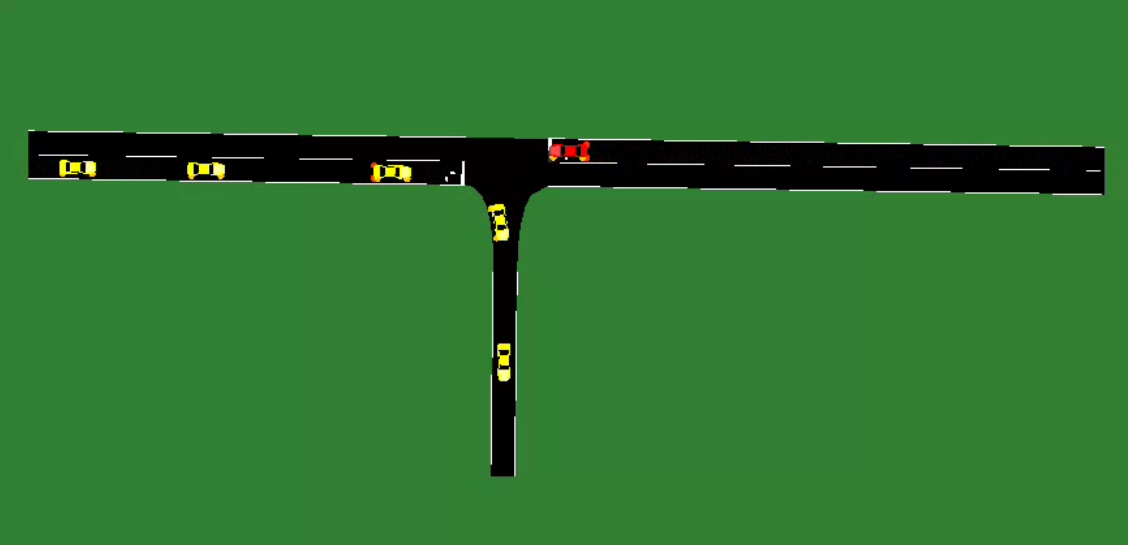
\includegraphics[width=\textwidth]{figures/Intersection_scenario.png}
        \textbf{(a)} Intersection scenario with the red vehicle
    \end{minipage}
    \hfill
    \begin{minipage}{0.48\textwidth}
        \centering
        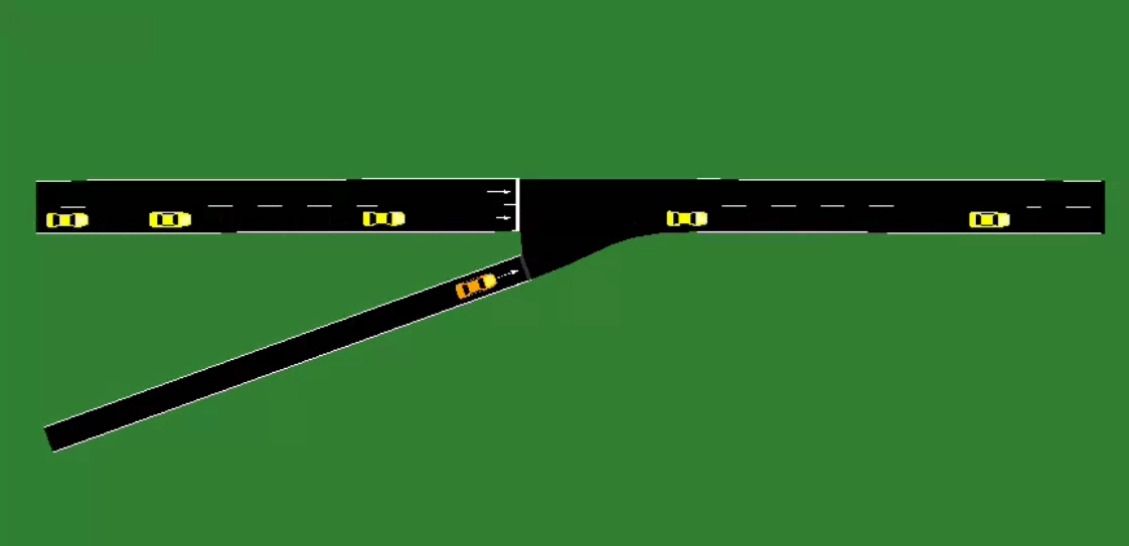
\includegraphics[width=\textwidth]{figures/Merging_scenario.png}
        \textbf{(b)} Merging scenario with the orange vehicle
    \end{minipage}

    \caption{SUMO traffic scenarios used in the project\cite{maad2025dynamic}.}
    \label{fig:traffic_scenarios}
\end{figure}

\noindent
These two scenarios are useful because they represent different types of driving decisions and allow the behavior of the learning agents to be tested under different traffic conditions.

\subsection{Agents and Experimental Setup}

The existing framework defines different agent configurations using the SUMO configuration file, vehicle ID, route edges, vehicle color, model path, and metric output path. In the codebase, the red agent is linked to the intersection scenario, while the orange agent is linked to the ramp merging scenario. The configuration also specifies where trained models and metrics are saved.

The original codebase already contained Q-Learning and DQN implementations. In this project, DDQN and PPO were added to the same experimental setup. DDQN was integrated using the DQN-style environment and training structure, while PPO required a separate environment wrapper and an actor-critic model. This makes it possible to test the added models under the same general simulation conditions as the previous agents.

\subsection{Training and Validation Pipeline}

The codebase is organized into separate scripts for each learning approach. The original framework includes training and validation files for Q-Learning and DQN, while additional scripts were added for DDQN and PPO. The main script is used to configure the selected agent, SUMO configuration file, vehicle ID, route edges, model path, metric output path, and number of episodes.

Each algorithm follows the same general execution flow in the codebase. A SUMO command is created, the environment wrapper is initialized, the agent is loaded or created, and the experiment is then executed episode by episode. After training, the learned model is saved either as a Q-table or as neural network weights, depending on the algorithm.

Figure~\ref{fig:training_validation_pipeline} summarizes the execution flow used by the training and validation scripts.

\begin{figure}[h]
    \centering
    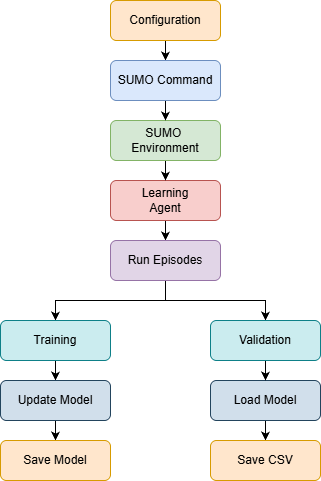
\includegraphics[width=0.45\textwidth]{figures/Diagram2.drawio.png}
    \caption{Training and validation pipeline used in the project codebase.}
    \label{fig:training_validation_pipeline}
\end{figure}

\noindent
The validation scripts reuse the saved models and store the resulting metrics in CSV files. These output files are later used to compare the agents in terms of reward, travel time, success, speed, collision-related information, and traffic impact.


\section{Algorithm Implementation}

This section presents the implementation structure of the learning algorithms used in the project. The existing codebase provided the baseline agents, including Q-Learning and DQN, while the additional work focused on implementing DDQN and PPO within the same SUMO-based experimental setup.

The purpose of this section is to explain how the algorithms are connected to the project structure. The main implementation differences are therefore described in terms of model structure, training process, validation process, and integration with the existing environment.

The section begins with the baseline implementations from the original framework, followed by the DDQN and PPO implementations added during this work.

\subsection{Baseline Implementations in the Existing Codebase}

The original codebase provided the baseline structure for running reinforcement learning experiments in SUMO. It already included environment wrappers, agent configuration files, training scripts, validation scripts, and metric collection tools. The framework was designed around controlled vehicle agents tested in traffic scenarios such as an intersection and a ramp merge, which are also described in the reference work by Maad et al. \cite{maad2025dynamic}.

The first baseline was the Q-Learning agent. In the existing implementation, this agent used the discrete state representation of the environment and stored the learned action values in a Q-table. The training script updated the table during interaction with the SUMO environment, while the validation script loaded the saved table and selected the action with the highest value for the current state.

The second baseline was the DQN agent. In this implementation, the agent used a neural network-based structure instead of a Q-table. The code included a policy network, a target network, replay memory, and saved model weights. This baseline was especially useful for the DDQN implementation, because DDQN could be integrated by keeping most of the DQN training structure and changing the target value calculation.

These baselines provided the main environment structure, training flow, validation flow, and metric-saving process used later for the DDQN and PPO implementations.


\subsection{DDQN Implementation}

The DDQN implementation was added as a deep value-based model using the existing DQN structure as a starting point. The same SUMO environment wrapper, state representation, action space, reward function, replay memory, and training loop style were kept in order to maintain consistency with the previous DQN baseline.

The DDQN agent uses two neural networks: a policy network and a target network. Both networks follow the same feed-forward architecture, with two hidden layers and ReLU activation functions. The policy network is used to select actions, while the target network is used to provide more stable target estimates during training.

The main implementation difference is introduced in the target Q-value calculation. In the DQN baseline, the target value is computed by taking the maximum Q-value from the target network. In DDQN, this step is separated into two parts: the policy network selects the best next action, and the target network evaluates the value of that selected action. This follows the main idea of Double DQN, which was introduced to reduce overestimation in action-value learning \cite{vanhasselt2016deep}.

The target used in the original Double DQN paper is defined as:

\[
Y_t^{DoubleDQN} =
R_{t+1} + \gamma Q\left(S_{t+1},
\arg\max_a Q(S_{t+1}, a; \theta_t);
\theta_t^{-}\right)
\]

where $\theta_t$ represents the parameters of the online network and
$\theta_t^{-}$ represents the parameters of the target network. In this
formulation, the online network is used to select the next action, while
the target network is used to evaluate the value of that selected action.
This separation is the main difference between DQN and DDQN and is used
to reduce overestimation in action-value learning \cite{vanhasselt2016deep}.


In the implementation, transitions are stored in replay memory as state, action, reward, next state, and done flag. During training, a batch of transitions is sampled from memory, the predicted Q-value is computed for the selected action, and the DDQN target is used to update the policy network. The target network is updated periodically by copying the weights from the policy network.

The DDQN model is trained using the same traffic scenarios and evaluation structure as the previous DQN agent. After training, the learned network weights are saved and later loaded during validation, where the agent selects actions using the trained policy without random exploration.

\subsection{PPO Implementation}

The PPO implementation was added as a separate actor-critic model. Unlike DDQN, which follows the structure of the existing DQN agent, PPO required a different implementation because it learns a policy directly instead of estimating Q-values for each action.

The PPO agent uses an actor-critic neural network. The shared layers first process the input state, and then the network is divided into two outputs. The actor outputs action probabilities, while the critic estimates the value of the current state. In this implementation, the state is converted into a one-hot vector before being passed to the network, since the PPO environment uses a discrete state representation.
Figure~\ref{fig:Diagram} shows the actor-critic structure used by the PPO agent.

\begin{figure}[h]
    \centering
    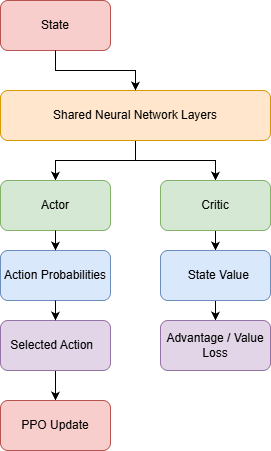
\includegraphics[width=0.35\textwidth]{figures/Diagram.drawio.png}
    \caption{Actor-critic structure used in the PPO implementation.}
    \label{fig:Diagram}
\end{figure}

\noindent
During training, the PPO agent samples actions from the probability distribution produced by the actor. For each step, the implementation stores the state, selected action, reward, terminal flag, log probability, and value estimate in a temporary trajectory memory. After one episode is collected, this memory is used to update the actor-critic network, and then it is cleared before the next episode.

The main PPO update is based on the clipped objective introduced by Schulman et al. \cite{schulman2017proximal}. The probability ratio between the new and old policies is computed as:

\[
r_t(\theta) =
\frac{\pi_\theta(a_t \mid s_t)}
{\pi_{\theta_{\text{old}}}(a_t \mid s_t)}
\]

The clipped objective is then written as:

\[
L^{CLIP}(\theta) =
\mathbf{E}_t
\left[
\min
\left(
r_t(\theta)\hat{A}_t,
\text{clip}(r_t(\theta), 1-\epsilon, 1+\epsilon)\hat{A}_t
\right)
\right]
\]

where \(r_t(\theta)\) is the policy probability ratio, \(\hat{A}_t\) is the advantage estimate, and \(\epsilon\) is the clipping parameter. In the implementation, this corresponds to comparing the unclipped objective with the clipped objective and using the smaller value for the actor loss. This limits large policy updates and helps keep the training process more stable.

The total loss combines the actor loss, critic loss, and entropy term. The critic loss improves the value prediction, while the entropy term encourages exploration by preventing the policy from becoming too deterministic too early. After the update, the PPO model weights are saved and later loaded during validation, where the action with the highest probability is selected.

\section{Experiments}

This section describes the experiments carried out to test the implemented agents within the existing SUMO framework. The aim was not to reproduce the full transfer learning and policy fusion experiments from the reference work, but to train and validate the added DDQN and PPO agents using the available scenario configurations.

The experiments were therefore organized around the same two traffic tasks used in the existing framework: the Red agent in the intersection scenario and the Orange agent in the ramp merge scenario. These scenarios provide the basis for testing whether the added algorithms can be integrated into the original training and validation pipeline.


\subsection{Implemented Agents}

The experiments focus on the agents implemented and integrated during this work. DDQN was added as a deep value-based agent using the existing DQN structure as a starting point. PPO was added as a separate actor-critic agent with its own training, validation, and environment files.

The original codebase already contained Q-Learning and DQN implementations, which served as baseline references. The added DDQN and PPO agents were connected to the same general experimental workflow, including SUMO configuration files, vehicle identifiers, model saving paths, and metric output files.

\subsection{Scenario Configuration}

The experiments were prepared using two scenario-agent configurations from the existing framework. The Red agent is associated with the intersection scenario and uses the vehicle identifier \texttt{v\_red}. The Orange agent is associated with the ramp merge scenario and uses the vehicle identifier \texttt{v\_orange}.

For the Red agent, the configuration is based on the intersection SUMO file and the route edges \texttt{('-E0', 'E1')}. For the Orange agent, the configuration is based on the ramp merge SUMO file and the route edges \texttt{('E1', 'E0.58')}. These scenario-agent pairings follow the same setup used in the reference framework by Maad et al. \cite{maad2025dynamic}.

The same scenario structure was used for the added DDQN and PPO agents, so that the new implementations could be tested within the existing training and validation pipeline.

\subsection{Training and Validation Runs}

For each implemented agent, the experiment consisted of a training run followed by a validation run. During training, the agent interacted with the SUMO environment and the learned model was saved after the training process. During validation, the saved model was loaded and tested without further learning.

The DDQN experiments saved the trained model as neural network weights and then loaded these weights during validation. The PPO experiments followed the same overall training-validation structure, but used the actor-critic model and the PPO-specific validation function. In both cases, the validation results were saved as CSV files containing the evaluation metrics used later for analysis.

This setup was used to verify that the added DDQN and PPO implementations could run inside the existing framework and produce training and validation outputs for the Red and Orange agent scenarios.

\noindent
The source code and experimental files for this project are available in the following GitHub repository:
\href{https://github.com/edonisa-dautaj/SUMO-RL-Autonomous-Vehicle-Coordination}{https://github.com/edonisa-dautaj/SUMO-RL-Autonomous-Vehicle-Coordination}.

\section{Results}

This section presents the validation results obtained for the implemented DDQN and PPO agents. The models were evaluated in the two main scenarios of the project: the Red agent in the intersection scenario and the Orange agent in the ramp merge scenario.

For DDQN, the validation results were stable enough to be reported quantitatively. For PPO, the implementation was completed and tested, but the validation behavior was less stable, especially for the Orange agent in the ramp merge scenario. Therefore, the PPO results are discussed as preliminary implementation results rather than as final optimized performance.

\begin{table}[H]
\centering
\caption{DDQN validation performance for the Red and Orange agents.}
\label{tab:ddqn_validation_results}
\vspace{0.2cm}
\begin{tabular}{|p{0.55\textwidth}|c|}
\hline
\textbf{Agent and Scenario} & \textbf{DDQN Success Rate} \\
\hline
Red agent in intersection & 97.4\% \\
\hline
Orange agent in merge & 93.8\% \\
\hline
\end{tabular}
\end{table}

\noindent
As shown in Table~\ref{tab:ddqn_validation_results}, the DDQN agent achieved high validation success rates in both evaluated scenarios. The Red agent reached 97.4% success in the intersection scenario, while the Orange agent reached 93.8% success in the ramp merge scenario. These results show that the existing DQN-based pipeline was successfully extended with DDQN and that the agent was able to learn stable behavior in both environments.

\begin{table}[H]
\centering
\caption{Additional DDQN validation metrics for the Red and Orange agents.}
\label{tab:ddqn_additional_metrics}
\vspace{0.2cm}
\begin{tabular}{|p{0.45\textwidth}|c|c|}
\hline
\textbf{Metric} & \textbf{Red Agent} & \textbf{Orange Agent} \\
\hline
Average reward & 2.50 & 2.48 \\
\hline
Average travel time (s) & 10.85 & 11.00 \\
\hline
Average speed (m/s) & 10.83 & 11.56 \\
\hline
Affected followers & 0.45 & 0.29 \\
\hline
Average deceleration (m/s$^2$) & 0.73 & 0.27 \\
\hline
\end{tabular}
\end{table}

\noindent
The additional DDQN metrics provide more detail about the behavior of the agents. Besides achieving high success rates, both agents completed the scenarios with reasonable travel times and average speeds. The affected follower and average deceleration values also indicate that the controlled vehicles had a limited impact on surrounding traffic during validation.

\noindent
PPO was also implemented and tested as an actor-critic policy-gradient method. The Red PPO agent produced promising validation behavior in the intersection scenario, showing that the implementation was able to learn useful driving actions. However, the Orange PPO agent in the ramp merge scenario was less stable. During deterministic validation, where the action with the highest probability was selected, the Orange agent often showed aggressive merging behavior and collided with surrounding vehicles. This suggests that the learned PPO policy was not yet robust enough for the ramp merge task.

\noindent
Additional tests showed that stochastic rollouts of the PPO policy could produce better behavior, but these were not used as the main validation result because the goal of validation was to evaluate the learned policy without additional exploration. For this reason, the PPO results are treated as preliminary. The implementation is functional and integrated into the SUMO framework, but further tuning would be required before making a strong final comparison with DDQN.




\section{Discussion}

The results show that the added algorithms could be integrated into the existing SUMO-based reinforcement learning framework. This is important because the main goal of the project was not to build a new simulation environment from the beginning, but to extend the existing reinforcement learning pipeline with additional deep reinforcement learning methods.

The DDQN implementation produced the most stable validation results in this work. Since DDQN was developed by adapting the existing DQN structure, it could be integrated into the current pipeline without major changes to the environment or simulation setup. The high validation success rates for both the Red agent in the intersection scenario and the Orange agent in the ramp merge scenario show that the DQN-based approach was extended successfully.

The PPO implementation was also successfully connected to the framework, but its results were less stable. The Red PPO agent showed promising behavior in the intersection scenario, which suggests that the actor-critic implementation was able to learn useful actions. However, the Orange PPO agent in the ramp merge scenario still showed limitations during deterministic validation. In several episodes, the agent selected aggressive merging behavior, which led to unsafe interactions with surrounding vehicles. For this reason, the PPO results should be interpreted as preliminary implementation results rather than final optimized performance.

The difference between the Red and Orange PPO behavior also shows that the ramp merge scenario is more sensitive to the learned policy. The Orange agent has to adapt its speed, choose a safe gap, and merge into the main traffic flow. This requires more precise decision-making than simply reaching the destination. The current PPO state representation and reward design may not provide enough information or guidance for the agent to consistently learn safe merging behavior.

The additional validation metrics help explain the agents' behavior beyond success rate alone. Success rate is the most direct measure of whether the vehicle completed the scenario safely, but metrics such as reward, travel time, average speed, affected followers, and average deceleration provide more detail about efficiency and traffic impact. For example, an agent may complete an episode successfully but still affect nearby vehicles or produce unnecessary braking. For this reason, these supporting metrics are useful when interpreting the quality of the learned behavior.

One limitation of this work is that the experiments focused only on training and validation of the added DDQN and PPO agents. The full zero-shot evaluation, transfer learning, fine-tuning, and policy fusion experiments from the original framework were not reproduced for the new models. Therefore, the results mainly show that DDQN and PPO can be implemented, trained, and tested within the existing SUMO framework, rather than proving their performance in all possible transfer settings.

Another limitation is that the PPO implementation was not fully optimized due to time constraints. Additional tuning of the PPO hyperparameters, state representation, reward function, and validation setup would be needed before making a stronger comparison with DDQN or with the original Q-Learning and DQN baselines. More scenarios, different traffic densities, and additional validation runs would also be needed to make stronger conclusions about generalization. Future work could use the implemented DDQN and PPO agents as a starting point for transfer learning experiments and for comparing value-based and policy-gradient methods in more complex traffic situations.





\section{Conclusion}

This paper presented the integration of additional deep reinforcement learning methods for autonomous vehicle coordination in SUMO. Starting from an existing framework that already included Q-Learning and DQN, the project added DDQN and PPO as new learning approaches.

DDQN was developed by building on the existing DQN structure, while PPO was implemented as a separate actor-critic model. Both methods were connected to the available SUMO scenarios: the Red agent in the intersection scenario and the Orange agent in the ramp merge scenario.

The DDQN implementation produced stable validation results and showed that the existing DQN-based pipeline could be extended successfully. PPO was also implemented and tested within the framework, and the Red PPO agent showed promising behavior in the intersection scenario. However, the Orange PPO agent in the ramp merge scenario remained less stable during deterministic validation, which shows that the PPO implementation still requires further improvement before it can be considered fully optimized.

Overall, the project shows that DDQN and PPO can be integrated into the existing SUMO simulation pipeline and used as a basis for autonomous vehicle decision-making experiments. However, the results also show that implementing a new reinforcement learning algorithm is not only a matter of adding the model, but also requires careful tuning of the state representation, reward function, action selection strategy, and validation setup.

Future work should first focus on improving the PPO implementation, especially for the ramp merge scenario. This could include refining the state representation so that the agent receives more useful information about nearby vehicles and safe merging gaps, adjusting the reward function to penalize unsafe merging behavior more effectively, and tuning PPO hyperparameters such as the learning rate, entropy coefficient, clipping value, and number of update epochs. Additional validation runs under different traffic densities would also be needed to better evaluate robustness and generalization.

Another important direction would be to extend the implemented DDQN and PPO agents to the transfer learning, fine-tuning, and policy fusion settings of the original framework. This would make it possible to study whether the added deep reinforcement learning methods can benefit from knowledge transfer between the Red intersection agent and the Orange ramp merge agent. Further work could also compare deterministic and stochastic policy evaluation for PPO in order to better understand how the learned policy behaves during validation.




\bibliographystyle{plain}
\bibliography{references}


\end{document}
